%%%%%%%%%%%%%%%%%%%%%%%%%%%%%%%%%%%%%%%%%%%%%%%%%%%%%%%%%%%%%%%%
% %
% Due Date %
% Andrew Gibson %
% ECE 351 lab, Section 53 %
% Lab 2 %
% Due 21 Feb 2023 %
% Step and Impulse Response of an RLC Bandpass Filter %
%https://github.com/gibs0630/ECE351\_Code %
%https://github.com/gibs0630/ECE351\_Reports %
% %
%%%%%%%%%%%%%%%%%%%%%%%%%%%%%%%%%%%%%%%%%%%%%%%%%%%%%%%%%%%%%%%%

\documentclass[12pt,a4paper]{article}
\usepackage[utf8]{inputenc}
\usepackage[greek,english]{babel}
\usepackage{alphabeta} 
\usepackage[pdftex]{graphicx}
\usepackage[top=1in, bottom=1in, left=1in, right=1in]{geometry}
\linespread{1.06}
\setlength{\parskip}{8pt plus2pt minus2pt}
\widowpenalty 10000
\clubpenalty 10000
\newcommand{\eat}[1]{}
\newcommand{\HRule}{\rule{\linewidth}{0.5mm}}
\usepackage[official]{eurosym}
\usepackage{enumitem}
\setlist{nolistsep,noitemsep}
\usepackage[hidelinks]{hyperref}
\usepackage{cite}
\usepackage{lipsum}


\newcommand{\Q}{\leavevmode\par\textbf {Q:}}
\newcommand{\A}{\par\textbf{A:} \normalfont}

\hypersetup{colorlinks=true, linkcolor=black, urlcolor=blue}

\begin{document}
%===========================================================
\begin{titlepage}
\begin{center}
% Top 
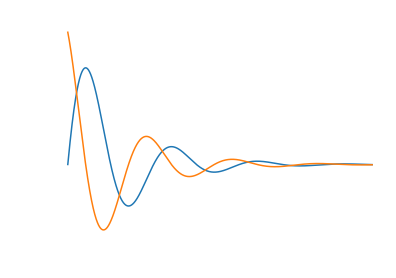
\includegraphics[width=0.55\textwidth]{titlepage_image.png}~\\[2cm]
% Title
\HRule \\[0.4cm]
{ \LARGE 
  \textbf{Project Report for ECE 351}\\[0.4cm]
  \emph{Lab 5: Step and Impulse Response of an RLC Bandpass Filter}\\[0.4cm]
}
\HRule \\[1.5cm]
% Author
{ \large
  Andrew Gibson \\[0.1cm]
 14 February 2023\\[0.1cm]
  \url{https://github.com/gibs0630/ECE351\_Code}\\[0.1cm]
  \url{https://github.com/gibs0630/ECE351\_Reports}\\[0.1cm]
  %#\texttt{user@cut.ac.cy}
}
\vfill
%\textsc{\Large Cyprus University of Technology}\\[0.4cm]\textsc{\large Department of Electrical Engineering,\\Computer Engineering \& Informatics}\\[0.4cm]
% Bottom
{\large }
 
\end{center}
\end{titlepage}
%\begin{abstract}
%\lipsum[1-2]
%\addtocontents{toc}{\protect\thispagestyle{empty}}
%\end{abstract}
\newpage
%===========================================================
\tableofcontents
\addtocontents{toc}{\protect\thispagestyle{empty}}
\newpage
\setcounter{page}{1}
%===========================================================
%===========================================================
\section{Introduction}\label{sec:intro}
When figuring out the output to a signal filter, it is useful to operate the math in the s domain (where algebra is easier) than working with derivatives and integrals. Once the impulse response function is found for that circuit, it becomes simpler to find how that signal will respond to a forcing function (aka input to the circuit).  If the signal is stable then some Laplace inverse computations can be skipped when finding the eventual state an input. Using signal synthesizer software these can be robustly modeled.

\section{Equations}\label{sec:lit-rev}
Formula's used
unit step function
\[
u(x) = \left\{
        \begin{array}{ll}
            0 & \quad t < 0 \\
            1 & \quad t \geq 0
        \end{array}
    \right.
\]
Final Value Theorem
\[
\lim _{s \to 0} \left [ s*F(s) \right] = \lim _{t \to \infty} \left [ f(t) \right]
\]
Laplace Transform pairs
\[e^{-\alpha t} cos(\omega t) u(t) = \frac {s+\alpha} {(s+\alpha)^2 + \omega}\]
\[e^{-\alpha t} sin(\omega t) u(t) = \frac {\omega} {(s+\alpha)^2 + \omega}\]

functions from lab


\[\omega_0 = \sqrt{ \frac {1} {C*L}-\left (\frac {1} {2*R*C} \right)^2}\]
\[\alpha_0 = \frac 1 {2*R*C}\] 
\[h_0 = e^{-\alpha_0*t}*\left(2*\alpha_0*\cos(\omega_0*t)-\frac {2*\alpha_0^2} {\omega_0}*\sin(\omega_0*t) \right)*u(t)\]


\[\omega_1 = \frac {1} {2} *\sqrt{\left| \left(\frac {1} {R*C} \right)^2-4*\left( \frac {1} {L*C} \right) \right|}\]
\[\alpha_1 = -1/(2*R*C)\]
\[|g| = \sqrt{\left(\frac {\omega_1} {R*C}\right)^2+\left(\frac{\alpha_1} {R*C} \right)^2}\]
\[\angle g = \arctan \left( \frac{\left (\frac {\omega_1}{R*C}\right)}{\left (\frac {\alpha_1} {R*C} \right)} \right)\]
\[h_1 = \frac{|g|}{\omega_1}*e^{\alpha_1*t}*\sin(\omega_1*t+\angle g)*u(t)\]


\section{Methodology}\label{sec:meth}
This lab had us analyze a circuit via hand calculations and then create a model in python to compare them.

\section{Results}\label{sec:res}
\subsection*{Part 1}

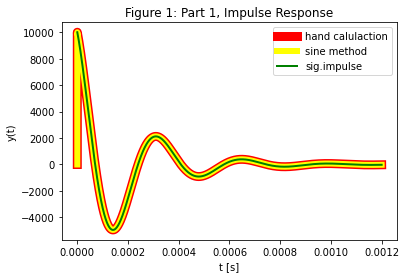
\includegraphics[width=0.55\textwidth]{Figure1.png}\\
The purpose producing Figure 1 to show that the answers from the hand calculation, through the sine method, and through using the signal library.


\subsection*{Part 2}
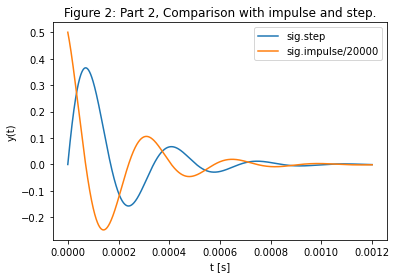
\includegraphics[width=0.55\textwidth]{Figure2.png}\\
Figure 2 shows the functions convolved with the unit step function.\\

\[
\frac {\frac {s} {R*C}} {s^2+\frac{s}{R*C} \frac{1}{C*L}}
\]

Do the poles prevent using the theorem? there are no poles in the positive real domain se we can use the theorem.

\[
\lim _{s \to 0} \left [ s*H(s) \right] = \lim _{t \to \infty} \left [ f(t) \right]
\]

\[
\lim _{s \to 0} \left [ s*H(s) \right] = \lim _{t \to \infty} \left [ f(t) \right]
\]

\[
\lim _{s \to 0} \left [ s*\frac {\frac {s} {R*C}} {s^2+\frac{s}{R*C}+ \frac{1}{C*L}} \right] = \lim _{t \to \infty} \left [ f(t) \right]
\]

\[
\lim _{s \to 0} \left [ s*\frac {\frac {s} {R*C}} {s^2+\frac{s}{R*C} +\frac{1}{C*L}} \right] = \lim _{t \to \infty} \left [ f(t) \right]
\]
there is no dividing  zero by zero so we can plug in zero.
\[
 0*\frac {\frac {0} {R*C}} {0^2+\frac{0}{R*C}+ \frac{1}{C*L}} = \lim _{t \to \infty} \left [ f(t) \right]
\]
\[
 0 = \lim _{t \to \infty} \left [ f(t) \right]
\]


The impulse response momentary jitters the circuit until it will resettle where the resistor will absorb the back and forth motion, diminishing the voltage until it reaches 0. The step function also will have the voltage diminish to zero as the inductor will slowly begin to act like an open circuit.
Also, the reason the impulse is 20000 times larger is because of the nature of the impulse (spontaneously large amount of voltage over a small time interval)where as the step is way smaller.both of they decaying at the same time makes sense as well as when taking the convolution of the impulse response function and the forcing function set to the step function, you will end up with the integral of the impulse response function, and the integral of e to the power with negative terms will decay at the same relative rate.



\section{Questions}\label{sec:res}


\Q 1. Explain the result of the Final Value Theorem from Part 2 Task 2 in terms of the physical circuit components.
\A 1. As time approaches infinity, you can measure longer wavelengths  that will have their own location on the s domain. The s domain is the the inverse of the wavelength. As time approaches infinity. The circuit will get more attenuated from the resistor which means that the lower s values  will get smaller magnitudes.  The oscillation between the Capacitor and the inductor do not play in the long term because of that attenuation.

\Q 2. Leave any feedback on the clarity of the expectations, instructions, and deliverables.
\A 2. The most difficult part was verifying that the code you typed in was in fact the code you calculated. single character off typos will cascade and make your output junk.  With the method of sines for finding the solution took algebra in a different direction but it got the same results if you forced a potential imaginary number to be real (numpy.sqrt(-1) will return NaN instead of j).



%\lipsum[7-8]\cite{knuthwebsite}
%===========================================================
%===========================================================
\bibliographystyle{ieeetr}
\bibliography{refs}
\end{document} 
Annotations











